\documentclass[a4paper]{book}
\usepackage{makeidx}
\usepackage{natbib}
\usepackage{graphicx}
\usepackage{multicol}
\usepackage{float}
\usepackage{listings}
\usepackage{color}
\usepackage{ifthen}
\usepackage[table]{xcolor}
\usepackage{textcomp}
\usepackage{alltt}
\usepackage{ifpdf}
\ifpdf
\usepackage[pdftex,
            pagebackref=true,
            colorlinks=true,
            linkcolor=blue,
            unicode
           ]{hyperref}
\else
\usepackage[ps2pdf,
            pagebackref=true,
            colorlinks=true,
            linkcolor=blue,
            unicode
           ]{hyperref}
\usepackage{pspicture}
\fi
\usepackage[utf8]{inputenc}
\usepackage{polski}
\usepackage[T1]{fontenc}

\usepackage{mathptmx}
\usepackage[scaled=.90]{helvet}
\usepackage{courier}
\usepackage{sectsty}
\usepackage[titles]{tocloft}
\usepackage{doxygen}
\lstset{language=C++,inputencoding=utf8,basicstyle=\footnotesize,breaklines=true,breakatwhitespace=true,tabsize=8,numbers=left }
\makeindex
\setcounter{tocdepth}{3}
\renewcommand{\footrulewidth}{0.4pt}
\renewcommand{\familydefault}{\sfdefault}
\hfuzz=15pt
\setlength{\emergencystretch}{15pt}
\hbadness=750
\tolerance=750
\begin{document}
\hypersetup{pageanchor=false,citecolor=blue}
\begin{titlepage}
\vspace*{7cm}
\begin{center}
{\Large stos\-\_\-kolejka }\\
\vspace*{1cm}
{\large \-Wygenerowano przez Doxygen 1.7.6.1}\\
\vspace*{0.5cm}
{\small Sun Mar 16 2014 22:27:27}\\
\end{center}
\end{titlepage}
\clearemptydoublepage
\pagenumbering{roman}
\tableofcontents
\clearemptydoublepage
\pagenumbering{arabic}
\hypersetup{pageanchor=true,citecolor=blue}
\chapter{\-Struktura katalogów}
\section{\-Katalogi}
\-Ta struktura katalogów jest posortowana jest z grubsza, choć nie całkowicie, alfabetycznie\-:\begin{DoxyCompactList}
\item \contentsline{section}{prj}{\pageref{dir_72ac3c5f818c04dc42fe82d0bf8fa612}}{}
\begin{DoxyCompactList}
\item \contentsline{section}{src}{\pageref{dir_ffb8ee22a3ecf475aaff9fbae649efc7}}{}
\end{DoxyCompactList}
\end{DoxyCompactList}

\chapter{\-Indeks klas}
\section{\-Lista klas}
\-Tutaj znajdują się klasy, struktury, unie i interfejsy wraz z ich krótkimi opisami\-:\begin{DoxyCompactList}
\item\contentsline{section}{\hyperlink{classczas}{czas} }{\pageref{classczas}}{}
\item\contentsline{section}{\hyperlink{structelement}{element} }{\pageref{structelement}}{}
\item\contentsline{section}{\hyperlink{classkolejka}{kolejka} }{\pageref{classkolejka}}{}
\item\contentsline{section}{\hyperlink{classstos}{stos} }{\pageref{classstos}}{}
\item\contentsline{section}{\hyperlink{classstos__l}{stos\-\_\-l} }{\pageref{classstos__l}}{}
\end{DoxyCompactList}

\chapter{\-Indeks plików}
\section{\-Lista plików}
\-Tutaj znajduje się lista wszystkich plików z ich krótkimi opisami\-:\begin{DoxyCompactList}
\item\contentsline{section}{prj/src/\hyperlink{generator_8cpp}{generator.\-cpp} }{\pageref{generator_8cpp}}{}
\item\contentsline{section}{prj/src/\hyperlink{generator_8hh}{generator.\-hh} }{\pageref{generator_8hh}}{}
\item\contentsline{section}{prj/src/\hyperlink{kolejka__lista_8cpp}{kolejka\-\_\-lista.\-cpp} }{\pageref{kolejka__lista_8cpp}}{}
\item\contentsline{section}{prj/src/\hyperlink{kolejka__lista_8hh}{kolejka\-\_\-lista.\-hh} }{\pageref{kolejka__lista_8hh}}{}
\item\contentsline{section}{prj/src/\hyperlink{main_8cpp}{main.\-cpp} }{\pageref{main_8cpp}}{}
\item\contentsline{section}{prj/src/\hyperlink{stoper_8hh}{stoper.\-hh} }{\pageref{stoper_8hh}}{}
\item\contentsline{section}{prj/src/\hyperlink{stos_8cpp}{stos.\-cpp} }{\pageref{stos_8cpp}}{}
\item\contentsline{section}{prj/src/\hyperlink{stos_8hh}{stos.\-hh} }{\pageref{stos_8hh}}{}
\item\contentsline{section}{prj/src/\hyperlink{stos__lista_8cpp}{stos\-\_\-lista.\-cpp} }{\pageref{stos__lista_8cpp}}{}
\item\contentsline{section}{prj/src/\hyperlink{stos__lista_8hh}{stos\-\_\-lista.\-hh} }{\pageref{stos__lista_8hh}}{}
\end{DoxyCompactList}

\chapter{\-Dokumentacja katalogów}
\hypertarget{dir_72ac3c5f818c04dc42fe82d0bf8fa612}{\section{\-Dokumentacja katalogu prj/}
\label{dir_72ac3c5f818c04dc42fe82d0bf8fa612}\index{\-Dokumentacja katalogu prj/@{\-Dokumentacja katalogu prj/}}
}
\-Directory dependency graph for prj/\-:\nopagebreak
\begin{figure}[H]
\begin{center}
\leavevmode
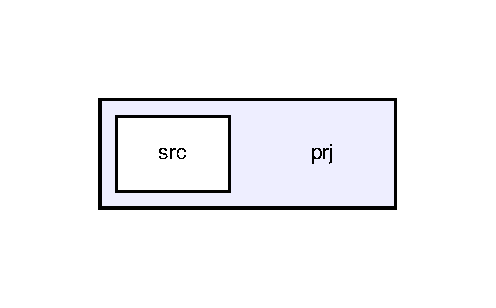
\includegraphics[width=238pt]{dir_72ac3c5f818c04dc42fe82d0bf8fa612_dep}
\end{center}
\end{figure}
\subsection*{\-Katalogi}
\begin{DoxyCompactItemize}
\item 
katalog \hyperlink{dir_ffb8ee22a3ecf475aaff9fbae649efc7}{src}
\end{DoxyCompactItemize}

\hypertarget{dir_ffb8ee22a3ecf475aaff9fbae649efc7}{\section{\-Dokumentacja katalogu prj/src/}
\label{dir_ffb8ee22a3ecf475aaff9fbae649efc7}\index{\-Dokumentacja katalogu prj/src/@{\-Dokumentacja katalogu prj/src/}}
}
\-Directory dependency graph for prj/src/\-:\nopagebreak
\begin{figure}[H]
\begin{center}
\leavevmode
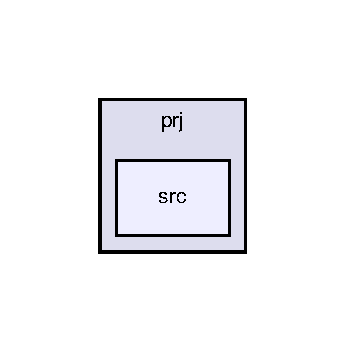
\includegraphics[width=166pt]{dir_ffb8ee22a3ecf475aaff9fbae649efc7_dep}
\end{center}
\end{figure}
\subsection*{\-Pliki}
\begin{DoxyCompactItemize}
\item 
plik \hyperlink{generator_8cpp}{generator.\-cpp}
\item 
plik \hyperlink{generator_8hh}{generator.\-hh}
\item 
plik \hyperlink{kolejka__lista_8cpp}{kolejka\-\_\-lista.\-cpp}
\item 
plik \hyperlink{kolejka__lista_8hh}{kolejka\-\_\-lista.\-hh}
\item 
plik \hyperlink{main_8cpp}{main.\-cpp}
\item 
plik \hyperlink{stoper_8hh}{stoper.\-hh}
\item 
plik \hyperlink{stos_8cpp}{stos.\-cpp}
\item 
plik \hyperlink{stos_8hh}{stos.\-hh}
\item 
plik \hyperlink{stos__lista_8cpp}{stos\-\_\-lista.\-cpp}
\item 
plik \hyperlink{stos__lista_8hh}{stos\-\_\-lista.\-hh}
\end{DoxyCompactItemize}

\chapter{\-Dokumentacja klas}
\hypertarget{classczas}{\section{\-Dokumentacja klasy czas}
\label{classczas}\index{czas@{czas}}
}


{\ttfamily \#include $<$stoper.\-hh$>$}

\subsection*{\-Metody publiczne}
\begin{DoxyCompactItemize}
\item 
void \hyperlink{classczas_a1e4c793526806f459e7f5c8c4a3ae29f}{start} ()
\begin{DoxyCompactList}\small\item\em start pomiaru zapisuje stan zegara \end{DoxyCompactList}\item 
void \hyperlink{classczas_a27f391e3c6bfb1f15f97c61bf403eb2d}{stop} ()
\begin{DoxyCompactList}\small\item\em koniec pomiaru zapisuje stan zegara \end{DoxyCompactList}\item 
double \hyperlink{classczas_a253df7797ca3cc3447d24c3c9477768e}{wynik} ()
\begin{DoxyCompactList}\small\item\em zwraca wynik pomiaru \end{DoxyCompactList}\item 
void \hyperlink{classczas_a53e5d67a7dd77239f2ef6ae0866e0596}{zapisz} (fstream \&\hyperlink{classczas_a253df7797ca3cc3447d24c3c9477768e}{wynik}, int rozmiar)
\begin{DoxyCompactList}\small\item\em zapisuje wynik do pliku \end{DoxyCompactList}\end{DoxyCompactItemize}
\subsection*{\-Atrybuty prywatne}
\begin{DoxyCompactItemize}
\item 
double \hyperlink{classczas_a1348fd4948270410b3087bb0318bd147}{time}
\item 
clock\-\_\-t \hyperlink{classczas_a3e75d47bf9beee497b56997b0b7be45c}{poczatek}
\item 
clock\-\_\-t \hyperlink{classczas_a65324dff284c101f2594b0b05b30399e}{koniec}
\end{DoxyCompactItemize}


\subsection{\-Opis szczegółowy}


\-Definicja w linii 19 pliku stoper.\-hh.



\subsection{\-Dokumentacja funkcji składowych}
\hypertarget{classczas_a1e4c793526806f459e7f5c8c4a3ae29f}{\index{czas@{czas}!start@{start}}
\index{start@{start}!czas@{czas}}
\subsubsection[{start}]{\setlength{\rightskip}{0pt plus 5cm}void {\bf czas\-::start} (
\begin{DoxyParamCaption}
{}
\end{DoxyParamCaption}
)\hspace{0.3cm}{\ttfamily  \mbox{[}inline\mbox{]}}}}\label{classczas_a1e4c793526806f459e7f5c8c4a3ae29f}


\-Definicja w linii 30 pliku stoper.\-hh.



\-Oto graf wywoływań tej funkcji\-:\nopagebreak
\begin{figure}[H]
\begin{center}
\leavevmode
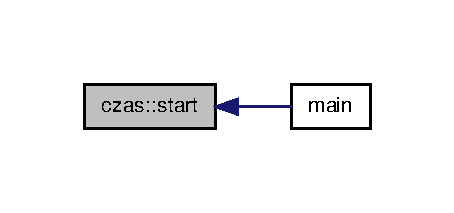
\includegraphics[width=218pt]{classczas_a1e4c793526806f459e7f5c8c4a3ae29f_icgraph}
\end{center}
\end{figure}


\hypertarget{classczas_a27f391e3c6bfb1f15f97c61bf403eb2d}{\index{czas@{czas}!stop@{stop}}
\index{stop@{stop}!czas@{czas}}
\subsubsection[{stop}]{\setlength{\rightskip}{0pt plus 5cm}void {\bf czas\-::stop} (
\begin{DoxyParamCaption}
{}
\end{DoxyParamCaption}
)\hspace{0.3cm}{\ttfamily  \mbox{[}inline\mbox{]}}}}\label{classczas_a27f391e3c6bfb1f15f97c61bf403eb2d}


\-Definicja w linii 38 pliku stoper.\-hh.



\-Oto graf wywoływań tej funkcji\-:\nopagebreak
\begin{figure}[H]
\begin{center}
\leavevmode
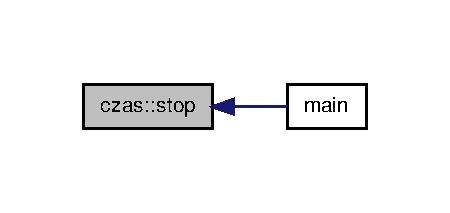
\includegraphics[width=216pt]{classczas_a27f391e3c6bfb1f15f97c61bf403eb2d_icgraph}
\end{center}
\end{figure}


\hypertarget{classczas_a253df7797ca3cc3447d24c3c9477768e}{\index{czas@{czas}!wynik@{wynik}}
\index{wynik@{wynik}!czas@{czas}}
\subsubsection[{wynik}]{\setlength{\rightskip}{0pt plus 5cm}double {\bf czas\-::wynik} (
\begin{DoxyParamCaption}
{}
\end{DoxyParamCaption}
)\hspace{0.3cm}{\ttfamily  \mbox{[}inline\mbox{]}}}}\label{classczas_a253df7797ca3cc3447d24c3c9477768e}
\begin{DoxyReturn}{\-Zwraca}
zwraca czas dzialania 
\end{DoxyReturn}


\-Definicja w linii 46 pliku stoper.\-hh.



\-Oto graf wywoływań tej funkcji\-:\nopagebreak
\begin{figure}[H]
\begin{center}
\leavevmode
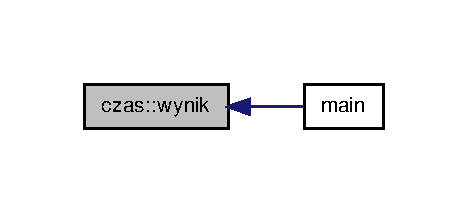
\includegraphics[width=224pt]{classczas_a253df7797ca3cc3447d24c3c9477768e_icgraph}
\end{center}
\end{figure}


\hypertarget{classczas_a53e5d67a7dd77239f2ef6ae0866e0596}{\index{czas@{czas}!zapisz@{zapisz}}
\index{zapisz@{zapisz}!czas@{czas}}
\subsubsection[{zapisz}]{\setlength{\rightskip}{0pt plus 5cm}void {\bf czas\-::zapisz} (
\begin{DoxyParamCaption}
\item[{fstream \&}]{wynik, }
\item[{int}]{rozmiar}
\end{DoxyParamCaption}
)\hspace{0.3cm}{\ttfamily  \mbox{[}inline\mbox{]}}}}\label{classczas_a53e5d67a7dd77239f2ef6ae0866e0596}

\begin{DoxyParams}{\-Parametry}
{\em wynik} & pomiaru \\
\hline
{\em rozmiar} & rozmiar problemu \\
\hline
\end{DoxyParams}


\-Definicja w linii 56 pliku stoper.\-hh.



\-Oto graf wywoływań tej funkcji\-:\nopagebreak
\begin{figure}[H]
\begin{center}
\leavevmode
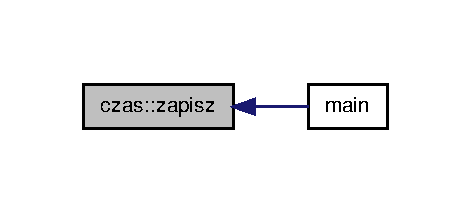
\includegraphics[width=226pt]{classczas_a53e5d67a7dd77239f2ef6ae0866e0596_icgraph}
\end{center}
\end{figure}




\subsection{\-Dokumentacja atrybutów składowych}
\hypertarget{classczas_a65324dff284c101f2594b0b05b30399e}{\index{czas@{czas}!koniec@{koniec}}
\index{koniec@{koniec}!czas@{czas}}
\subsubsection[{koniec}]{\setlength{\rightskip}{0pt plus 5cm}clock\-\_\-t {\bf czas\-::koniec}\hspace{0.3cm}{\ttfamily  \mbox{[}private\mbox{]}}}}\label{classczas_a65324dff284c101f2594b0b05b30399e}


\-Definicja w linii 24 pliku stoper.\-hh.

\hypertarget{classczas_a3e75d47bf9beee497b56997b0b7be45c}{\index{czas@{czas}!poczatek@{poczatek}}
\index{poczatek@{poczatek}!czas@{czas}}
\subsubsection[{poczatek}]{\setlength{\rightskip}{0pt plus 5cm}clock\-\_\-t {\bf czas\-::poczatek}\hspace{0.3cm}{\ttfamily  \mbox{[}private\mbox{]}}}}\label{classczas_a3e75d47bf9beee497b56997b0b7be45c}


\-Definicja w linii 24 pliku stoper.\-hh.

\hypertarget{classczas_a1348fd4948270410b3087bb0318bd147}{\index{czas@{czas}!time@{time}}
\index{time@{time}!czas@{czas}}
\subsubsection[{time}]{\setlength{\rightskip}{0pt plus 5cm}double {\bf czas\-::time}\hspace{0.3cm}{\ttfamily  \mbox{[}private\mbox{]}}}}\label{classczas_a1348fd4948270410b3087bb0318bd147}


\-Definicja w linii 23 pliku stoper.\-hh.



\-Dokumentacja dla tej klasy została wygenerowana z pliku\-:\begin{DoxyCompactItemize}
\item 
prj/src/\hyperlink{stoper_8hh}{stoper.\-hh}\end{DoxyCompactItemize}

\hypertarget{structelement}{\section{\-Dokumentacja struktury element}
\label{structelement}\index{element@{element}}
}


{\ttfamily \#include $<$kolejka\-\_\-lista.\-hh$>$}



\-Diagram współpracy dla element\-:\nopagebreak
\begin{figure}[H]
\begin{center}
\leavevmode
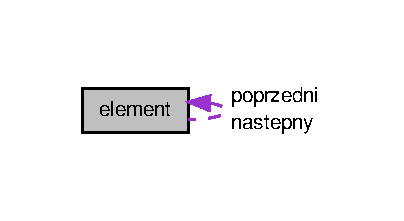
\includegraphics[width=194pt]{structelement__coll__graph}
\end{center}
\end{figure}
\subsection*{\-Atrybuty publiczne}
\begin{DoxyCompactItemize}
\item 
\hyperlink{structelement}{element} $\ast$ \hyperlink{structelement_ab6df52b0e5cfa7c4998a2ab74a8ef53e}{nastepny}
\item 
int \hyperlink{structelement_a4e4b66f785b98647b0ecbc85ec23d270}{dana}
\item 
\hyperlink{structelement}{element} $\ast$ \hyperlink{structelement_ab29a484726350416708a843bc30aa4fa}{poprzedni}
\end{DoxyCompactItemize}


\subsection{\-Opis szczegółowy}


\-Definicja w linii 14 pliku kolejka\-\_\-lista.\-hh.



\subsection{\-Dokumentacja atrybutów składowych}
\hypertarget{structelement_a4e4b66f785b98647b0ecbc85ec23d270}{\index{element@{element}!dana@{dana}}
\index{dana@{dana}!element@{element}}
\subsubsection[{dana}]{\setlength{\rightskip}{0pt plus 5cm}int {\bf element\-::dana}}}\label{structelement_a4e4b66f785b98647b0ecbc85ec23d270}


\-Definicja w linii 17 pliku kolejka\-\_\-lista.\-hh.

\hypertarget{structelement_ab6df52b0e5cfa7c4998a2ab74a8ef53e}{\index{element@{element}!nastepny@{nastepny}}
\index{nastepny@{nastepny}!element@{element}}
\subsubsection[{nastepny}]{\setlength{\rightskip}{0pt plus 5cm}{\bf element}$\ast$ {\bf element\-::nastepny}}}\label{structelement_ab6df52b0e5cfa7c4998a2ab74a8ef53e}


\-Definicja w linii 16 pliku kolejka\-\_\-lista.\-hh.

\hypertarget{structelement_ab29a484726350416708a843bc30aa4fa}{\index{element@{element}!poprzedni@{poprzedni}}
\index{poprzedni@{poprzedni}!element@{element}}
\subsubsection[{poprzedni}]{\setlength{\rightskip}{0pt plus 5cm}{\bf element}$\ast$ {\bf element\-::poprzedni}}}\label{structelement_ab29a484726350416708a843bc30aa4fa}


\-Definicja w linii 21 pliku stos\-\_\-lista.\-hh.



\-Dokumentacja dla tej struktury została wygenerowana z plików\-:\begin{DoxyCompactItemize}
\item 
prj/src/\hyperlink{kolejka__lista_8hh}{kolejka\-\_\-lista.\-hh}\item 
prj/src/\hyperlink{stos__lista_8hh}{stos\-\_\-lista.\-hh}\end{DoxyCompactItemize}

\hypertarget{classkolejka}{\section{\-Dokumentacja klasy kolejka}
\label{classkolejka}\index{kolejka@{kolejka}}
}


{\ttfamily \#include $<$kolejka\-\_\-lista.\-hh$>$}



\-Diagram współpracy dla kolejka\-:\nopagebreak
\begin{figure}[H]
\begin{center}
\leavevmode
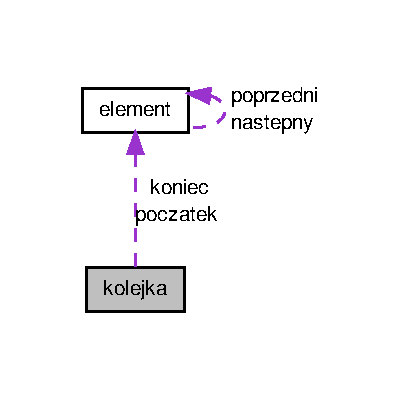
\includegraphics[width=194pt]{classkolejka__coll__graph}
\end{center}
\end{figure}
\subsection*{\-Metody publiczne}
\begin{DoxyCompactItemize}
\item 
\hyperlink{classkolejka_ae9205d86a1f136649fac28615878729c}{kolejka} ()
\begin{DoxyCompactList}\small\item\em konstruktor klasy kolejka, zeruje stałą rozmiar; \end{DoxyCompactList}\item 
void \hyperlink{classkolejka_a090a263c1b0e37c3e447ffbf577da590}{push} (int dana)
\begin{DoxyCompactList}\small\item\em dodaje na koniec kolejki zmienna \end{DoxyCompactList}\item 
int \hyperlink{classkolejka_afdf5d84aff3c9500e696d3b6df092ace}{pop} ()
\begin{DoxyCompactList}\small\item\em zdejmuje pierwszy element z kolejki \end{DoxyCompactList}\item 
bool \hyperlink{classkolejka_adf983aef6073856cba88f5d75b9cd084}{isempty} ()
\item 
int \hyperlink{classkolejka_a74bf7134474481c349d08d0fd321390e}{size} ()
\end{DoxyCompactItemize}
\subsection*{\-Atrybuty prywatne}
\begin{DoxyCompactItemize}
\item 
\hyperlink{structelement}{element} $\ast$ \hyperlink{classkolejka_a71d1822dbeb8c1b76339c2429f0527c2}{poczatek}
\item 
\hyperlink{structelement}{element} $\ast$ \hyperlink{classkolejka_a60ae9fd137487acc5dc01dbe467fc7cc}{koniec}
\item 
int \hyperlink{classkolejka_a0fe33a7248ca72a87c55ab9e56c0e172}{rozmiar}
\end{DoxyCompactItemize}


\subsection{\-Opis szczegółowy}


\-Definicja w linii 26 pliku kolejka\-\_\-lista.\-hh.



\subsection{\-Dokumentacja konstruktora i destruktora}
\hypertarget{classkolejka_ae9205d86a1f136649fac28615878729c}{\index{kolejka@{kolejka}!kolejka@{kolejka}}
\index{kolejka@{kolejka}!kolejka@{kolejka}}
\subsubsection[{kolejka}]{\setlength{\rightskip}{0pt plus 5cm}{\bf kolejka\-::kolejka} (
\begin{DoxyParamCaption}
{}
\end{DoxyParamCaption}
)}}\label{classkolejka_ae9205d86a1f136649fac28615878729c}


\-Definicja w linii 11 pliku kolejka\-\_\-lista.\-cpp.



\subsection{\-Dokumentacja funkcji składowych}
\hypertarget{classkolejka_adf983aef6073856cba88f5d75b9cd084}{\index{kolejka@{kolejka}!isempty@{isempty}}
\index{isempty@{isempty}!kolejka@{kolejka}}
\subsubsection[{isempty}]{\setlength{\rightskip}{0pt plus 5cm}bool {\bf kolejka\-::isempty} (
\begin{DoxyParamCaption}
{}
\end{DoxyParamCaption}
)}}\label{classkolejka_adf983aef6073856cba88f5d75b9cd084}
\begin{DoxyReturn}{\-Zwraca}
1 jesli pusta jesli pelna 
\end{DoxyReturn}


\-Definicja w linii 64 pliku kolejka\-\_\-lista.\-cpp.



\-Oto graf wywoływań tej funkcji\-:\nopagebreak
\begin{figure}[H]
\begin{center}
\leavevmode
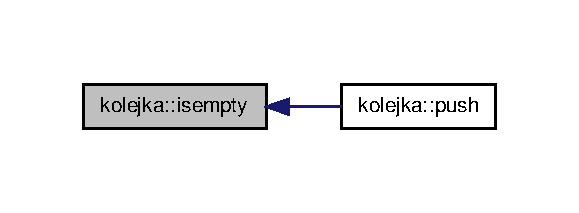
\includegraphics[width=278pt]{classkolejka_adf983aef6073856cba88f5d75b9cd084_icgraph}
\end{center}
\end{figure}


\hypertarget{classkolejka_afdf5d84aff3c9500e696d3b6df092ace}{\index{kolejka@{kolejka}!pop@{pop}}
\index{pop@{pop}!kolejka@{kolejka}}
\subsubsection[{pop}]{\setlength{\rightskip}{0pt plus 5cm}int {\bf kolejka\-::pop} (
\begin{DoxyParamCaption}
{}
\end{DoxyParamCaption}
)}}\label{classkolejka_afdf5d84aff3c9500e696d3b6df092ace}
\begin{DoxyReturn}{\-Zwraca}
zwraca element znajdujacy sie na poczatku kolejki 
\end{DoxyReturn}


\-Definicja w linii 38 pliku kolejka\-\_\-lista.\-cpp.

\hypertarget{classkolejka_a090a263c1b0e37c3e447ffbf577da590}{\index{kolejka@{kolejka}!push@{push}}
\index{push@{push}!kolejka@{kolejka}}
\subsubsection[{push}]{\setlength{\rightskip}{0pt plus 5cm}void {\bf kolejka\-::push} (
\begin{DoxyParamCaption}
\item[{int}]{dana}
\end{DoxyParamCaption}
)}}\label{classkolejka_a090a263c1b0e37c3e447ffbf577da590}

\begin{DoxyParams}{\-Parametry}
{\em dana} & zmienna ktora zostanie dodana \\
\hline
\end{DoxyParams}


\-Definicja w linii 20 pliku kolejka\-\_\-lista.\-cpp.



\-Oto graf wywołań dla tej funkcji\-:\nopagebreak
\begin{figure}[H]
\begin{center}
\leavevmode
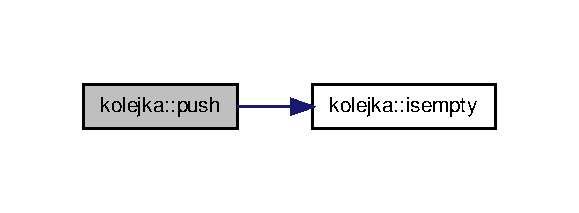
\includegraphics[width=278pt]{classkolejka_a090a263c1b0e37c3e447ffbf577da590_cgraph}
\end{center}
\end{figure}


\hypertarget{classkolejka_a74bf7134474481c349d08d0fd321390e}{\index{kolejka@{kolejka}!size@{size}}
\index{size@{size}!kolejka@{kolejka}}
\subsubsection[{size}]{\setlength{\rightskip}{0pt plus 5cm}int {\bf kolejka\-::size} (
\begin{DoxyParamCaption}
{}
\end{DoxyParamCaption}
)}}\label{classkolejka_a74bf7134474481c349d08d0fd321390e}
\begin{DoxyReturn}{\-Zwraca}
zwraca rozmiar kolejki 
\end{DoxyReturn}


\-Definicja w linii 55 pliku kolejka\-\_\-lista.\-cpp.



\subsection{\-Dokumentacja atrybutów składowych}
\hypertarget{classkolejka_a60ae9fd137487acc5dc01dbe467fc7cc}{\index{kolejka@{kolejka}!koniec@{koniec}}
\index{koniec@{koniec}!kolejka@{kolejka}}
\subsubsection[{koniec}]{\setlength{\rightskip}{0pt plus 5cm}{\bf element}$\ast$ {\bf kolejka\-::koniec}\hspace{0.3cm}{\ttfamily  \mbox{[}private\mbox{]}}}}\label{classkolejka_a60ae9fd137487acc5dc01dbe467fc7cc}


\-Definicja w linii 30 pliku kolejka\-\_\-lista.\-hh.

\hypertarget{classkolejka_a71d1822dbeb8c1b76339c2429f0527c2}{\index{kolejka@{kolejka}!poczatek@{poczatek}}
\index{poczatek@{poczatek}!kolejka@{kolejka}}
\subsubsection[{poczatek}]{\setlength{\rightskip}{0pt plus 5cm}{\bf element}$\ast$ {\bf kolejka\-::poczatek}\hspace{0.3cm}{\ttfamily  \mbox{[}private\mbox{]}}}}\label{classkolejka_a71d1822dbeb8c1b76339c2429f0527c2}


\-Definicja w linii 29 pliku kolejka\-\_\-lista.\-hh.

\hypertarget{classkolejka_a0fe33a7248ca72a87c55ab9e56c0e172}{\index{kolejka@{kolejka}!rozmiar@{rozmiar}}
\index{rozmiar@{rozmiar}!kolejka@{kolejka}}
\subsubsection[{rozmiar}]{\setlength{\rightskip}{0pt plus 5cm}int {\bf kolejka\-::rozmiar}\hspace{0.3cm}{\ttfamily  \mbox{[}private\mbox{]}}}}\label{classkolejka_a0fe33a7248ca72a87c55ab9e56c0e172}


\-Definicja w linii 31 pliku kolejka\-\_\-lista.\-hh.



\-Dokumentacja dla tej klasy została wygenerowana z plików\-:\begin{DoxyCompactItemize}
\item 
prj/src/\hyperlink{kolejka__lista_8hh}{kolejka\-\_\-lista.\-hh}\item 
prj/src/\hyperlink{kolejka__lista_8cpp}{kolejka\-\_\-lista.\-cpp}\end{DoxyCompactItemize}

\hypertarget{classstos}{\section{\-Dokumentacja klasy stos}
\label{classstos}\index{stos@{stos}}
}


{\ttfamily \#include $<$stos.\-hh$>$}

\subsection*{\-Metody publiczne}
\begin{DoxyCompactItemize}
\item 
\hyperlink{classstos_afb387ac69250038334f6d8099b6a2421}{stos} ()
\begin{DoxyCompactList}\small\item\em \-Konstruktor. \end{DoxyCompactList}\item 
void \hyperlink{classstos_a501f0a03fece3b29c32939355cd46154}{push} (int dana)
\begin{DoxyCompactList}\small\item\em dodaje zmienn do stosu \end{DoxyCompactList}\item 
int \hyperlink{classstos_a809ccf5ceabaa74dbd7c84c78102cded}{pop} ()
\begin{DoxyCompactList}\small\item\em sciaga zmienna ze stosu \end{DoxyCompactList}\item 
bool \hyperlink{classstos_a28f9b17c72b4a91221e4bae54e169895}{isempty} ()
\begin{DoxyCompactList}\small\item\em sprawdza czy jest cos na stosie; \end{DoxyCompactList}\item 
int \hyperlink{classstos_a47fcfe525e580ceb48080b33ab3d53de}{size} ()
\begin{DoxyCompactList}\small\item\em sprawdza ilosc danych \end{DoxyCompactList}\end{DoxyCompactItemize}
\subsection*{\-Metody prywatne}
\begin{DoxyCompactItemize}
\item 
void \hyperlink{classstos_aaf0cbb2759166f5c8ade9db7edd12e71}{zwieksz\-\_\-dwa} ()
\begin{DoxyCompactList}\small\item\em zweikasza dwukrotnie rozmiar stosu gdy brakuje miejsca \end{DoxyCompactList}\item 
void \hyperlink{classstos_a46a2e2a17327297ca70b40ff39524cef}{zwieksz\-\_\-o\-\_\-1} ()
\begin{DoxyCompactList}\small\item\em zwieksza rozmiar tablicy o 1 \end{DoxyCompactList}\item 
void \hyperlink{classstos_a7eaf47bc9feeea0777e07f89d0d304cf}{zwieksz} ()
\item 
void \hyperlink{classstos_ae5ace69c31d9de2f24eb872895216bf3}{kopiuj} (int $\ast$s\-\_\-tab)
\begin{DoxyCompactList}\small\item\em kopiuje zawartosc jednej tablicy do drugiej \end{DoxyCompactList}\item 
void \hyperlink{classstos_aeabdfcdd334943a4a22a6f095bd7a873}{zmniejsz} ()
\begin{DoxyCompactList}\small\item\em \-Zmniejsza rozmar tablicy dwukrotnie. \end{DoxyCompactList}\end{DoxyCompactItemize}
\subsection*{\-Atrybuty prywatne}
\begin{DoxyCompactItemize}
\item 
int $\ast$ \hyperlink{classstos_a71155717d44c2156515be8edb1139358}{tab}
\item 
int \hyperlink{classstos_aaccd7c15d97e23313862cca67f56f3ab}{rozmiar}
\item 
int \hyperlink{classstos_a5769bde313093eb321b0b15111c7ec35}{aktualna}
\end{DoxyCompactItemize}


\subsection{\-Opis szczegółowy}


\-Definicja w linii 25 pliku stos.\-hh.



\subsection{\-Dokumentacja konstruktora i destruktora}
\hypertarget{classstos_afb387ac69250038334f6d8099b6a2421}{\index{stos@{stos}!stos@{stos}}
\index{stos@{stos}!stos@{stos}}
\subsubsection[{stos}]{\setlength{\rightskip}{0pt plus 5cm}{\bf stos\-::stos} (
\begin{DoxyParamCaption}
{}
\end{DoxyParamCaption}
)}}\label{classstos_afb387ac69250038334f6d8099b6a2421}
\-Zeruje zmienna rozmiar i aktualna 

\-Definicja w linii 86 pliku stos.\-cpp.



\subsection{\-Dokumentacja funkcji składowych}
\hypertarget{classstos_a28f9b17c72b4a91221e4bae54e169895}{\index{stos@{stos}!isempty@{isempty}}
\index{isempty@{isempty}!stos@{stos}}
\subsubsection[{isempty}]{\setlength{\rightskip}{0pt plus 5cm}bool {\bf stos\-::isempty} (
\begin{DoxyParamCaption}
{}
\end{DoxyParamCaption}
)}}\label{classstos_a28f9b17c72b4a91221e4bae54e169895}
\begin{DoxyReturn}{\-Zwraca}
zwraca 1 gdy pusta 
\end{DoxyReturn}


\-Definicja w linii 124 pliku stos.\-cpp.



\-Oto graf wywoływań tej funkcji\-:\nopagebreak
\begin{figure}[H]
\begin{center}
\leavevmode
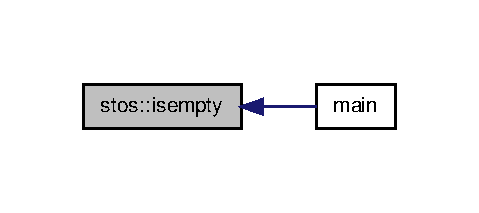
\includegraphics[width=230pt]{classstos_a28f9b17c72b4a91221e4bae54e169895_icgraph}
\end{center}
\end{figure}


\hypertarget{classstos_ae5ace69c31d9de2f24eb872895216bf3}{\index{stos@{stos}!kopiuj@{kopiuj}}
\index{kopiuj@{kopiuj}!stos@{stos}}
\subsubsection[{kopiuj}]{\setlength{\rightskip}{0pt plus 5cm}void {\bf stos\-::kopiuj} (
\begin{DoxyParamCaption}
\item[{int $\ast$}]{s\-\_\-tab}
\end{DoxyParamCaption}
)\hspace{0.3cm}{\ttfamily  \mbox{[}private\mbox{]}}}}\label{classstos_ae5ace69c31d9de2f24eb872895216bf3}

\begin{DoxyParams}{\-Parametry}
{\em s\-\_\-tab} & \\
\hline
\end{DoxyParams}


\-Definicja w linii 18 pliku stos.\-cpp.



\-Oto graf wywoływań tej funkcji\-:\nopagebreak
\begin{figure}[H]
\begin{center}
\leavevmode
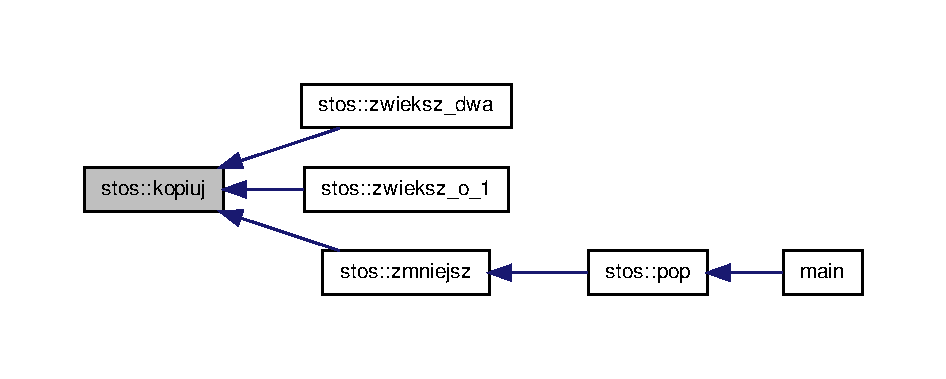
\includegraphics[width=350pt]{classstos_ae5ace69c31d9de2f24eb872895216bf3_icgraph}
\end{center}
\end{figure}


\hypertarget{classstos_a809ccf5ceabaa74dbd7c84c78102cded}{\index{stos@{stos}!pop@{pop}}
\index{pop@{pop}!stos@{stos}}
\subsubsection[{pop}]{\setlength{\rightskip}{0pt plus 5cm}int {\bf stos\-::pop} (
\begin{DoxyParamCaption}
{}
\end{DoxyParamCaption}
)}}\label{classstos_a809ccf5ceabaa74dbd7c84c78102cded}
\-Sprawdza rowniez rozmiar tablicy. \-Jesli tablica zajeta w 1/4 zmniejsza jej rozmiar o polowe. \begin{DoxyReturn}{\-Zwraca}

\end{DoxyReturn}


\-Definicja w linii 110 pliku stos.\-cpp.



\-Oto graf wywołań dla tej funkcji\-:\nopagebreak
\begin{figure}[H]
\begin{center}
\leavevmode
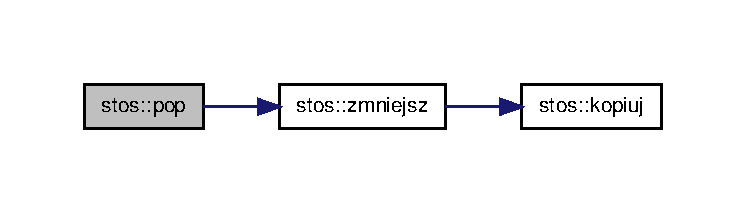
\includegraphics[width=350pt]{classstos_a809ccf5ceabaa74dbd7c84c78102cded_cgraph}
\end{center}
\end{figure}




\-Oto graf wywoływań tej funkcji\-:\nopagebreak
\begin{figure}[H]
\begin{center}
\leavevmode
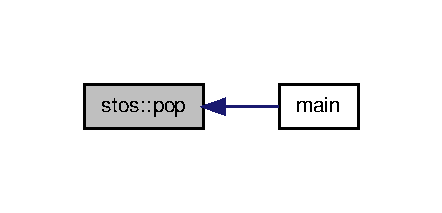
\includegraphics[width=212pt]{classstos_a809ccf5ceabaa74dbd7c84c78102cded_icgraph}
\end{center}
\end{figure}


\hypertarget{classstos_a501f0a03fece3b29c32939355cd46154}{\index{stos@{stos}!push@{push}}
\index{push@{push}!stos@{stos}}
\subsubsection[{push}]{\setlength{\rightskip}{0pt plus 5cm}void {\bf stos\-::push} (
\begin{DoxyParamCaption}
\item[{int}]{dana}
\end{DoxyParamCaption}
)}}\label{classstos_a501f0a03fece3b29c32939355cd46154}
funkcja sprawdza czy tablica nie jest zapelniona i dodaje zienna.

\-Jesli tablica pelna wywoluje funkcje zwiekszajaca jej rozmiar

\-Z\-W\-I\-E\-K\-S\-Z-\/ definicja w pliku \hyperlink{stos_8hh}{stos.\-hh} 
\begin{DoxyParams}{\-Parametry}
{\em dana} & \\
\hline
\end{DoxyParams}


\-Definicja w linii 98 pliku stos.\-cpp.



\-Oto graf wywoływań tej funkcji\-:\nopagebreak
\begin{figure}[H]
\begin{center}
\leavevmode
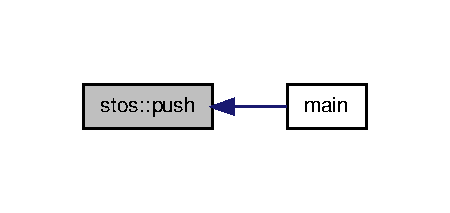
\includegraphics[width=216pt]{classstos_a501f0a03fece3b29c32939355cd46154_icgraph}
\end{center}
\end{figure}


\hypertarget{classstos_a47fcfe525e580ceb48080b33ab3d53de}{\index{stos@{stos}!size@{size}}
\index{size@{size}!stos@{stos}}
\subsubsection[{size}]{\setlength{\rightskip}{0pt plus 5cm}int {\bf stos\-::size} (
\begin{DoxyParamCaption}
{}
\end{DoxyParamCaption}
)}}\label{classstos_a47fcfe525e580ceb48080b33ab3d53de}
\begin{DoxyReturn}{\-Zwraca}
ilosc zmiennych w stosie; 
\end{DoxyReturn}


\-Definicja w linii 134 pliku stos.\-cpp.



\-Oto graf wywoływań tej funkcji\-:\nopagebreak
\begin{figure}[H]
\begin{center}
\leavevmode
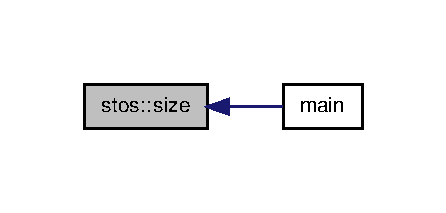
\includegraphics[width=214pt]{classstos_a47fcfe525e580ceb48080b33ab3d53de_icgraph}
\end{center}
\end{figure}


\hypertarget{classstos_aeabdfcdd334943a4a22a6f095bd7a873}{\index{stos@{stos}!zmniejsz@{zmniejsz}}
\index{zmniejsz@{zmniejsz}!stos@{stos}}
\subsubsection[{zmniejsz}]{\setlength{\rightskip}{0pt plus 5cm}void {\bf stos\-::zmniejsz} (
\begin{DoxyParamCaption}
{}
\end{DoxyParamCaption}
)\hspace{0.3cm}{\ttfamily  \mbox{[}private\mbox{]}}}}\label{classstos_aeabdfcdd334943a4a22a6f095bd7a873}
gdy stos zajmuje 1/4 rozmiaru tablicy jest ona zmniejszana o 1/2 

\-Definicja w linii 61 pliku stos.\-cpp.



\-Oto graf wywołań dla tej funkcji\-:\nopagebreak
\begin{figure}[H]
\begin{center}
\leavevmode
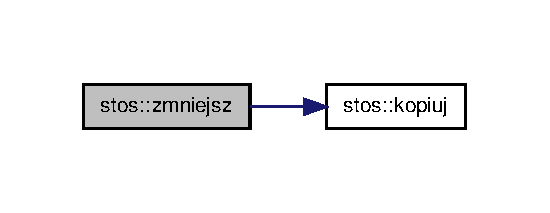
\includegraphics[width=264pt]{classstos_aeabdfcdd334943a4a22a6f095bd7a873_cgraph}
\end{center}
\end{figure}




\-Oto graf wywoływań tej funkcji\-:\nopagebreak
\begin{figure}[H]
\begin{center}
\leavevmode
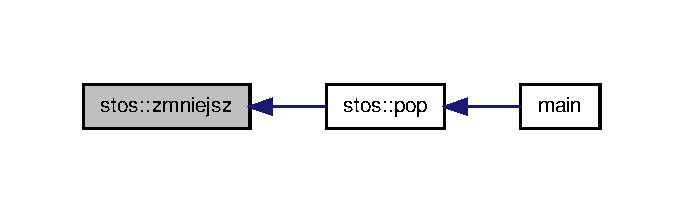
\includegraphics[width=328pt]{classstos_aeabdfcdd334943a4a22a6f095bd7a873_icgraph}
\end{center}
\end{figure}


\hypertarget{classstos_a7eaf47bc9feeea0777e07f89d0d304cf}{\index{stos@{stos}!zwieksz@{zwieksz}}
\index{zwieksz@{zwieksz}!stos@{stos}}
\subsubsection[{zwieksz}]{\setlength{\rightskip}{0pt plus 5cm}void {\bf stos\-::zwieksz} (
\begin{DoxyParamCaption}
{}
\end{DoxyParamCaption}
)\hspace{0.3cm}{\ttfamily  \mbox{[}private\mbox{]}}}}\label{classstos_a7eaf47bc9feeea0777e07f89d0d304cf}
\hypertarget{classstos_aaf0cbb2759166f5c8ade9db7edd12e71}{\index{stos@{stos}!zwieksz\-\_\-dwa@{zwieksz\-\_\-dwa}}
\index{zwieksz\-\_\-dwa@{zwieksz\-\_\-dwa}!stos@{stos}}
\subsubsection[{zwieksz\-\_\-dwa}]{\setlength{\rightskip}{0pt plus 5cm}void {\bf stos\-::zwieksz\-\_\-dwa} (
\begin{DoxyParamCaption}
{}
\end{DoxyParamCaption}
)\hspace{0.3cm}{\ttfamily  \mbox{[}private\mbox{]}}}}\label{classstos_aaf0cbb2759166f5c8ade9db7edd12e71}


\-Definicja w linii 25 pliku stos.\-cpp.



\-Oto graf wywołań dla tej funkcji\-:\nopagebreak
\begin{figure}[H]
\begin{center}
\leavevmode
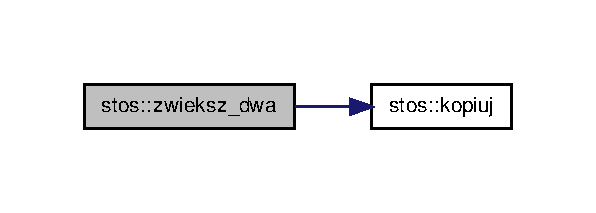
\includegraphics[width=286pt]{classstos_aaf0cbb2759166f5c8ade9db7edd12e71_cgraph}
\end{center}
\end{figure}


\hypertarget{classstos_a46a2e2a17327297ca70b40ff39524cef}{\index{stos@{stos}!zwieksz\-\_\-o\-\_\-1@{zwieksz\-\_\-o\-\_\-1}}
\index{zwieksz\-\_\-o\-\_\-1@{zwieksz\-\_\-o\-\_\-1}!stos@{stos}}
\subsubsection[{zwieksz\-\_\-o\-\_\-1}]{\setlength{\rightskip}{0pt plus 5cm}void {\bf stos\-::zwieksz\-\_\-o\-\_\-1} (
\begin{DoxyParamCaption}
{}
\end{DoxyParamCaption}
)\hspace{0.3cm}{\ttfamily  \mbox{[}private\mbox{]}}}}\label{classstos_a46a2e2a17327297ca70b40ff39524cef}


\-Definicja w linii 46 pliku stos.\-cpp.



\-Oto graf wywołań dla tej funkcji\-:\nopagebreak
\begin{figure}[H]
\begin{center}
\leavevmode
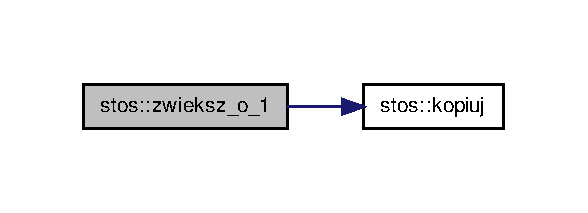
\includegraphics[width=282pt]{classstos_a46a2e2a17327297ca70b40ff39524cef_cgraph}
\end{center}
\end{figure}




\subsection{\-Dokumentacja atrybutów składowych}
\hypertarget{classstos_a5769bde313093eb321b0b15111c7ec35}{\index{stos@{stos}!aktualna@{aktualna}}
\index{aktualna@{aktualna}!stos@{stos}}
\subsubsection[{aktualna}]{\setlength{\rightskip}{0pt plus 5cm}int {\bf stos\-::aktualna}\hspace{0.3cm}{\ttfamily  \mbox{[}private\mbox{]}}}}\label{classstos_a5769bde313093eb321b0b15111c7ec35}


\-Definicja w linii 30 pliku stos.\-hh.

\hypertarget{classstos_aaccd7c15d97e23313862cca67f56f3ab}{\index{stos@{stos}!rozmiar@{rozmiar}}
\index{rozmiar@{rozmiar}!stos@{stos}}
\subsubsection[{rozmiar}]{\setlength{\rightskip}{0pt plus 5cm}int {\bf stos\-::rozmiar}\hspace{0.3cm}{\ttfamily  \mbox{[}private\mbox{]}}}}\label{classstos_aaccd7c15d97e23313862cca67f56f3ab}


\-Definicja w linii 29 pliku stos.\-hh.

\hypertarget{classstos_a71155717d44c2156515be8edb1139358}{\index{stos@{stos}!tab@{tab}}
\index{tab@{tab}!stos@{stos}}
\subsubsection[{tab}]{\setlength{\rightskip}{0pt plus 5cm}int$\ast$ {\bf stos\-::tab}\hspace{0.3cm}{\ttfamily  \mbox{[}private\mbox{]}}}}\label{classstos_a71155717d44c2156515be8edb1139358}


\-Definicja w linii 28 pliku stos.\-hh.



\-Dokumentacja dla tej klasy została wygenerowana z plików\-:\begin{DoxyCompactItemize}
\item 
prj/src/\hyperlink{stos_8hh}{stos.\-hh}\item 
prj/src/\hyperlink{stos_8cpp}{stos.\-cpp}\end{DoxyCompactItemize}

\hypertarget{classstos__l}{\section{\-Dokumentacja klasy stos\-\_\-l}
\label{classstos__l}\index{stos\-\_\-l@{stos\-\_\-l}}
}


{\ttfamily \#include $<$stos\-\_\-lista.\-hh$>$}



\-Diagram współpracy dla stos\-\_\-l\-:\nopagebreak
\begin{figure}[H]
\begin{center}
\leavevmode
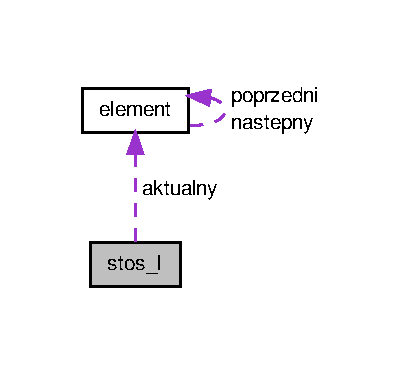
\includegraphics[width=194pt]{classstos__l__coll__graph}
\end{center}
\end{figure}
\subsection*{\-Metody publiczne}
\begin{DoxyCompactItemize}
\item 
\hyperlink{classstos__l_a817f8251137659e6d2ec081a84ea7041}{stos\-\_\-l} ()
\begin{DoxyCompactList}\small\item\em konstruktor zeruje zmienna rozmiar \end{DoxyCompactList}\item 
void \hyperlink{classstos__l_abf3d6a7f9835928a68998e9afc569ce8}{push} (int dana)
\item 
int \hyperlink{classstos__l_a83201bb86938e636121af57fa989f763}{pop} ()
\begin{DoxyCompactList}\small\item\em sciaga zmienna ze stosu \end{DoxyCompactList}\item 
bool \hyperlink{classstos__l_adeab314853e583fd3e6acc50167fcba2}{isempty} ()
\begin{DoxyCompactList}\small\item\em sprawdza czy stos jest pusty \end{DoxyCompactList}\item 
int \hyperlink{classstos__l_a3f517d1349edbae56ca94b431baab318}{size} ()
\begin{DoxyCompactList}\small\item\em sprawdza rozmiar stosu \end{DoxyCompactList}\end{DoxyCompactItemize}
\subsection*{\-Atrybuty prywatne}
\begin{DoxyCompactItemize}
\item 
\hyperlink{structelement}{element} $\ast$ \hyperlink{classstos__l_ac11dcea9266fd7258405656624cfc1f3}{aktualny}
\item 
int \hyperlink{classstos__l_a2194604d2193df66d042756db760d1ff}{rozmiar}
\end{DoxyCompactItemize}


\subsection{\-Opis szczegółowy}


\-Definicja w linii 27 pliku stos\-\_\-lista.\-hh.



\subsection{\-Dokumentacja konstruktora i destruktora}
\hypertarget{classstos__l_a817f8251137659e6d2ec081a84ea7041}{\index{stos\-\_\-l@{stos\-\_\-l}!stos\-\_\-l@{stos\-\_\-l}}
\index{stos\-\_\-l@{stos\-\_\-l}!stos_l@{stos\-\_\-l}}
\subsubsection[{stos\-\_\-l}]{\setlength{\rightskip}{0pt plus 5cm}{\bf stos\-\_\-l\-::stos\-\_\-l} (
\begin{DoxyParamCaption}
{}
\end{DoxyParamCaption}
)}}\label{classstos__l_a817f8251137659e6d2ec081a84ea7041}


\-Definicja w linii 14 pliku stos\-\_\-lista.\-cpp.



\subsection{\-Dokumentacja funkcji składowych}
\hypertarget{classstos__l_adeab314853e583fd3e6acc50167fcba2}{\index{stos\-\_\-l@{stos\-\_\-l}!isempty@{isempty}}
\index{isempty@{isempty}!stos_l@{stos\-\_\-l}}
\subsubsection[{isempty}]{\setlength{\rightskip}{0pt plus 5cm}bool {\bf stos\-\_\-l\-::isempty} (
\begin{DoxyParamCaption}
{}
\end{DoxyParamCaption}
)}}\label{classstos__l_adeab314853e583fd3e6acc50167fcba2}
\begin{DoxyReturn}{\-Zwraca}
1 pusty 0 pelny 
\end{DoxyReturn}


\-Definicja w linii 70 pliku stos\-\_\-lista.\-cpp.

\hypertarget{classstos__l_a83201bb86938e636121af57fa989f763}{\index{stos\-\_\-l@{stos\-\_\-l}!pop@{pop}}
\index{pop@{pop}!stos_l@{stos\-\_\-l}}
\subsubsection[{pop}]{\setlength{\rightskip}{0pt plus 5cm}int {\bf stos\-\_\-l\-::pop} (
\begin{DoxyParamCaption}
{}
\end{DoxyParamCaption}
)}}\label{classstos__l_a83201bb86938e636121af57fa989f763}
\begin{DoxyReturn}{\-Zwraca}
zmienna zdjeta ze stosu 
\end{DoxyReturn}


\-Definicja w linii 45 pliku stos\-\_\-lista.\-cpp.

\hypertarget{classstos__l_abf3d6a7f9835928a68998e9afc569ce8}{\index{stos\-\_\-l@{stos\-\_\-l}!push@{push}}
\index{push@{push}!stos_l@{stos\-\_\-l}}
\subsubsection[{push}]{\setlength{\rightskip}{0pt plus 5cm}void {\bf stos\-\_\-l\-::push} (
\begin{DoxyParamCaption}
\item[{int}]{dana}
\end{DoxyParamCaption}
)}}\label{classstos__l_abf3d6a7f9835928a68998e9afc569ce8}
dodaje zmienna na szczty stosu 
\begin{DoxyParams}{\-Parametry}
{\em dana} & zmienna do dodania \\
\hline
\end{DoxyParams}


\-Definicja w linii 23 pliku stos\-\_\-lista.\-cpp.

\hypertarget{classstos__l_a3f517d1349edbae56ca94b431baab318}{\index{stos\-\_\-l@{stos\-\_\-l}!size@{size}}
\index{size@{size}!stos_l@{stos\-\_\-l}}
\subsubsection[{size}]{\setlength{\rightskip}{0pt plus 5cm}int {\bf stos\-\_\-l\-::size} (
\begin{DoxyParamCaption}
{}
\end{DoxyParamCaption}
)}}\label{classstos__l_a3f517d1349edbae56ca94b431baab318}
\begin{DoxyReturn}{\-Zwraca}
rozmiar stosu 
\end{DoxyReturn}


\-Definicja w linii 61 pliku stos\-\_\-lista.\-cpp.



\subsection{\-Dokumentacja atrybutów składowych}
\hypertarget{classstos__l_ac11dcea9266fd7258405656624cfc1f3}{\index{stos\-\_\-l@{stos\-\_\-l}!aktualny@{aktualny}}
\index{aktualny@{aktualny}!stos_l@{stos\-\_\-l}}
\subsubsection[{aktualny}]{\setlength{\rightskip}{0pt plus 5cm}{\bf element}$\ast$ {\bf stos\-\_\-l\-::aktualny}\hspace{0.3cm}{\ttfamily  \mbox{[}private\mbox{]}}}}\label{classstos__l_ac11dcea9266fd7258405656624cfc1f3}


\-Definicja w linii 30 pliku stos\-\_\-lista.\-hh.

\hypertarget{classstos__l_a2194604d2193df66d042756db760d1ff}{\index{stos\-\_\-l@{stos\-\_\-l}!rozmiar@{rozmiar}}
\index{rozmiar@{rozmiar}!stos_l@{stos\-\_\-l}}
\subsubsection[{rozmiar}]{\setlength{\rightskip}{0pt plus 5cm}int {\bf stos\-\_\-l\-::rozmiar}\hspace{0.3cm}{\ttfamily  \mbox{[}private\mbox{]}}}}\label{classstos__l_a2194604d2193df66d042756db760d1ff}


\-Definicja w linii 31 pliku stos\-\_\-lista.\-hh.



\-Dokumentacja dla tej klasy została wygenerowana z plików\-:\begin{DoxyCompactItemize}
\item 
prj/src/\hyperlink{stos__lista_8hh}{stos\-\_\-lista.\-hh}\item 
prj/src/\hyperlink{stos__lista_8cpp}{stos\-\_\-lista.\-cpp}\end{DoxyCompactItemize}

\chapter{\-Dokumentacja plików}
\hypertarget{generator_8cpp}{\section{\-Dokumentacja pliku prj/src/generator.cpp}
\label{generator_8cpp}\index{prj/src/generator.\-cpp@{prj/src/generator.\-cpp}}
}
{\ttfamily \#include \char`\"{}generator.\-hh\char`\"{}}\*
\-Wykres zależności załączania dla generator.\-cpp\-:\nopagebreak
\begin{figure}[H]
\begin{center}
\leavevmode
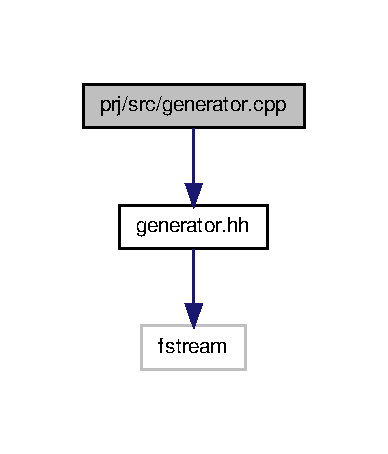
\includegraphics[width=186pt]{generator_8cpp__incl}
\end{center}
\end{figure}
\subsection*{\-Funkcje}
\begin{DoxyCompactItemize}
\item 
void \hyperlink{generator_8cpp_a8a338f908bb9996d5b01aab4439e8a56}{generuj} (char $\ast$nazwa, int rozmiar)
\begin{DoxyCompactList}\small\item\em generuje plik $\ast$.txt o zadanej ilosci danych i nazwie \end{DoxyCompactList}\end{DoxyCompactItemize}


\subsection{\-Dokumentacja funkcji}
\hypertarget{generator_8cpp_a8a338f908bb9996d5b01aab4439e8a56}{\index{generator.\-cpp@{generator.\-cpp}!generuj@{generuj}}
\index{generuj@{generuj}!generator.cpp@{generator.\-cpp}}
\subsubsection[{generuj}]{\setlength{\rightskip}{0pt plus 5cm}void {\bf generuj} (
\begin{DoxyParamCaption}
\item[{char $\ast$}]{nazwa, }
\item[{int}]{rozmiar}
\end{DoxyParamCaption}
)}}\label{generator_8cpp_a8a338f908bb9996d5b01aab4439e8a56}
\-W pliku umieszczane sa liczby naturalne od 1 wzwyrz w pierwszym wierszu umieszczana jest liczba mowiaca o ilosci wierszy danych. 
\begin{DoxyParams}{\-Parametry}
{\em nazwa} & -\/ utworzonego pliku \\
\hline
{\em rozmiar} & -\/ ilosc wierszy sanych \\
\hline
\end{DoxyParams}


\-Definicja w linii 19 pliku generator.\-cpp.



\-Oto graf wywoływań tej funkcji\-:\nopagebreak
\begin{figure}[H]
\begin{center}
\leavevmode
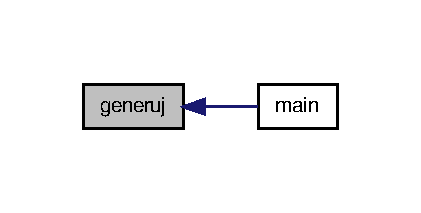
\includegraphics[width=202pt]{generator_8cpp_a8a338f908bb9996d5b01aab4439e8a56_icgraph}
\end{center}
\end{figure}



\hypertarget{generator_8hh}{\section{\-Dokumentacja pliku prj/src/generator.hh}
\label{generator_8hh}\index{prj/src/generator.\-hh@{prj/src/generator.\-hh}}
}
{\ttfamily \#include $<$fstream$>$}\*
\-Wykres zależności załączania dla generator.\-hh\-:\nopagebreak
\begin{figure}[H]
\begin{center}
\leavevmode
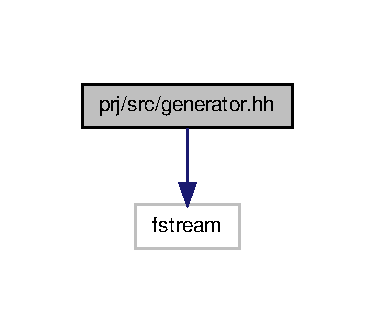
\includegraphics[width=180pt]{generator_8hh__incl}
\end{center}
\end{figure}
\-Ten wykres pokazuje, które pliki bezpośrednio lub pośrednio załączają ten plik\-:\nopagebreak
\begin{figure}[H]
\begin{center}
\leavevmode
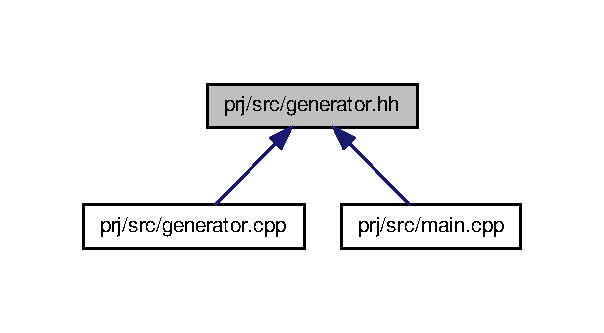
\includegraphics[width=290pt]{generator_8hh__dep__incl}
\end{center}
\end{figure}
\subsection*{\-Funkcje}
\begin{DoxyCompactItemize}
\item 
void \hyperlink{generator_8hh_a8a338f908bb9996d5b01aab4439e8a56}{generuj} (char $\ast$nazwa, int rozmiar)
\begin{DoxyCompactList}\small\item\em generuje plik $\ast$.txt o zadanej ilosci danych i nazwie \end{DoxyCompactList}\end{DoxyCompactItemize}


\subsection{\-Dokumentacja funkcji}
\hypertarget{generator_8hh_a8a338f908bb9996d5b01aab4439e8a56}{\index{generator.\-hh@{generator.\-hh}!generuj@{generuj}}
\index{generuj@{generuj}!generator.hh@{generator.\-hh}}
\subsubsection[{generuj}]{\setlength{\rightskip}{0pt plus 5cm}void {\bf generuj} (
\begin{DoxyParamCaption}
\item[{char $\ast$}]{nazwa, }
\item[{int}]{rozmiar}
\end{DoxyParamCaption}
)}}\label{generator_8hh_a8a338f908bb9996d5b01aab4439e8a56}
\-W pliku umieszczane sa liczby naturalne od 1 wzwyrz w pierwszym wierszu umieszczana jest liczba mowiaca o ilosci wierszy danych. 
\begin{DoxyParams}{\-Parametry}
{\em nazwa} & -\/ utworzonego pliku \\
\hline
{\em rozmiar} & -\/ ilosc wierszy sanych \\
\hline
\end{DoxyParams}


\-Definicja w linii 19 pliku generator.\-cpp.



\-Oto graf wywoływań tej funkcji\-:\nopagebreak
\begin{figure}[H]
\begin{center}
\leavevmode
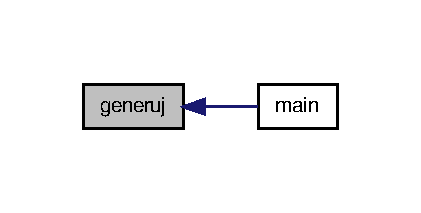
\includegraphics[width=202pt]{generator_8hh_a8a338f908bb9996d5b01aab4439e8a56_icgraph}
\end{center}
\end{figure}



\hypertarget{kolejka__lista_8cpp}{\section{\-Dokumentacja pliku prj/src/kolejka\-\_\-lista.cpp}
\label{kolejka__lista_8cpp}\index{prj/src/kolejka\-\_\-lista.\-cpp@{prj/src/kolejka\-\_\-lista.\-cpp}}
}
{\ttfamily \#include \char`\"{}kolejka\-\_\-lista.\-hh\char`\"{}}\*
\-Wykres zależności załączania dla kolejka\-\_\-lista.\-cpp\-:\nopagebreak
\begin{figure}[H]
\begin{center}
\leavevmode
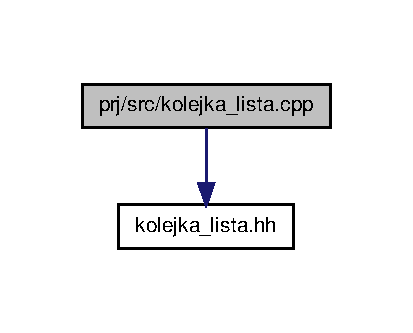
\includegraphics[width=198pt]{kolejka__lista_8cpp__incl}
\end{center}
\end{figure}

\hypertarget{kolejka__lista_8hh}{\section{\-Dokumentacja pliku prj/src/kolejka\-\_\-lista.hh}
\label{kolejka__lista_8hh}\index{prj/src/kolejka\-\_\-lista.\-hh@{prj/src/kolejka\-\_\-lista.\-hh}}
}
\-Ten wykres pokazuje, które pliki bezpośrednio lub pośrednio załączają ten plik\-:\nopagebreak
\begin{figure}[H]
\begin{center}
\leavevmode
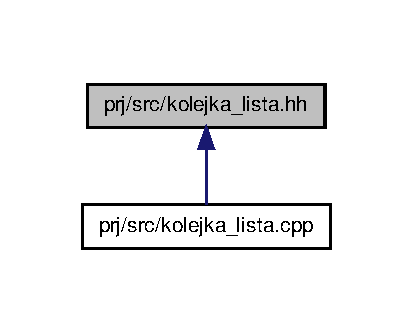
\includegraphics[width=198pt]{kolejka__lista_8hh__dep__incl}
\end{center}
\end{figure}
\subsection*{\-Komponenty}
\begin{DoxyCompactItemize}
\item 
struct \hyperlink{structelement}{element}
\item 
class \hyperlink{classkolejka}{kolejka}
\end{DoxyCompactItemize}

\hypertarget{main_8cpp}{\section{\-Dokumentacja pliku prj/src/main.cpp}
\label{main_8cpp}\index{prj/src/main.\-cpp@{prj/src/main.\-cpp}}
}
{\ttfamily \#include $<$iostream$>$}\*
{\ttfamily \#include \char`\"{}stos.\-hh\char`\"{}}\*
{\ttfamily \#include \char`\"{}stos\-\_\-lista.\-hh\char`\"{}}\*
{\ttfamily \#include \char`\"{}generator.\-hh\char`\"{}}\*
{\ttfamily \#include \char`\"{}stoper.\-hh\char`\"{}}\*
\-Wykres zależności załączania dla main.\-cpp\-:\nopagebreak
\begin{figure}[H]
\begin{center}
\leavevmode
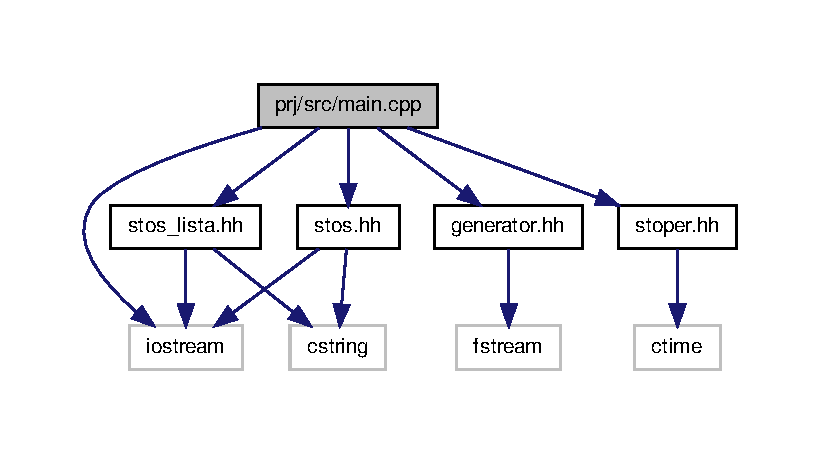
\includegraphics[width=350pt]{main_8cpp__incl}
\end{center}
\end{figure}
\subsection*{\-Funkcje}
\begin{DoxyCompactItemize}
\item 
int \hyperlink{main_8cpp_ae66f6b31b5ad750f1fe042a706a4e3d4}{main} ()
\end{DoxyCompactItemize}


\subsection{\-Dokumentacja funkcji}
\hypertarget{main_8cpp_ae66f6b31b5ad750f1fe042a706a4e3d4}{\index{main.\-cpp@{main.\-cpp}!main@{main}}
\index{main@{main}!main.cpp@{main.\-cpp}}
\subsubsection[{main}]{\setlength{\rightskip}{0pt plus 5cm}int {\bf main} (
\begin{DoxyParamCaption}
{}
\end{DoxyParamCaption}
)}}\label{main_8cpp_ae66f6b31b5ad750f1fe042a706a4e3d4}


\-Definicja w linii 17 pliku main.\-cpp.



\-Oto graf wywołań dla tej funkcji\-:\nopagebreak
\begin{figure}[H]
\begin{center}
\leavevmode
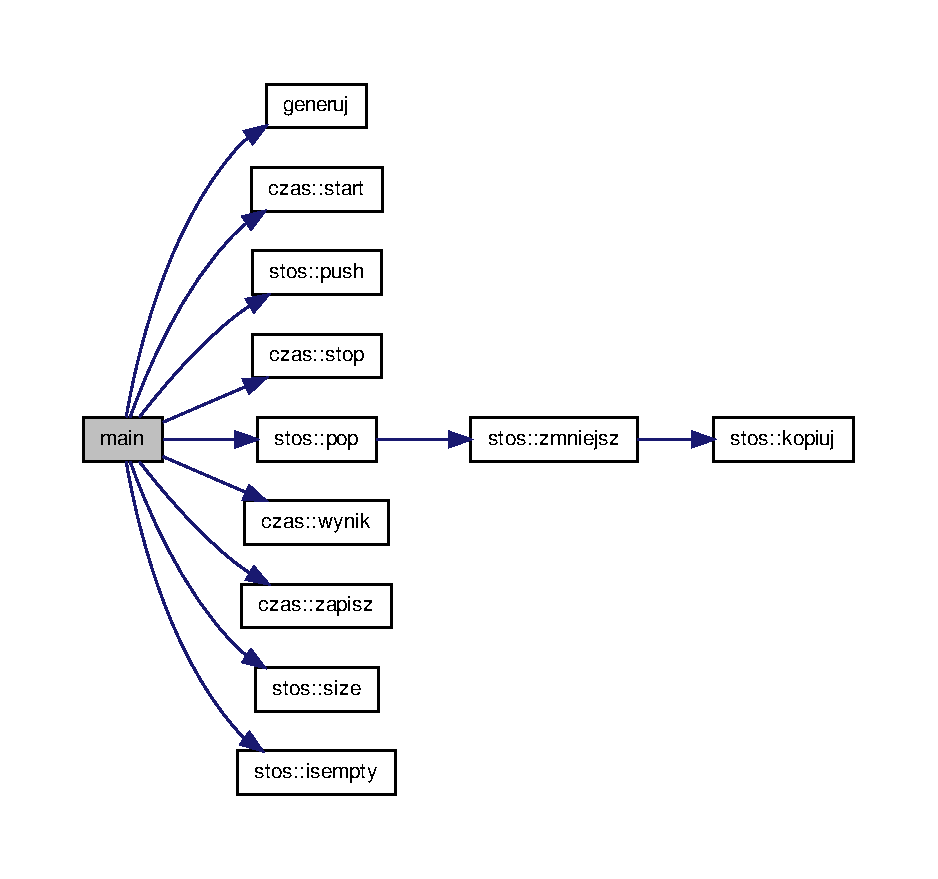
\includegraphics[width=350pt]{main_8cpp_ae66f6b31b5ad750f1fe042a706a4e3d4_cgraph}
\end{center}
\end{figure}



\hypertarget{stoper_8hh}{\section{\-Dokumentacja pliku prj/src/stoper.hh}
\label{stoper_8hh}\index{prj/src/stoper.\-hh@{prj/src/stoper.\-hh}}
}
{\ttfamily \#include $<$ctime$>$}\*
\-Wykres zależności załączania dla stoper.\-hh\-:\nopagebreak
\begin{figure}[H]
\begin{center}
\leavevmode
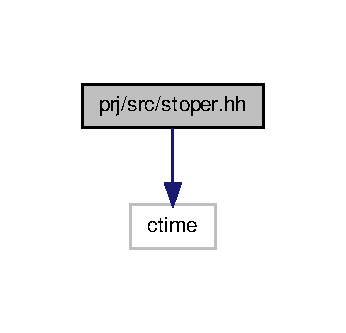
\includegraphics[width=166pt]{stoper_8hh__incl}
\end{center}
\end{figure}
\-Ten wykres pokazuje, które pliki bezpośrednio lub pośrednio załączają ten plik\-:\nopagebreak
\begin{figure}[H]
\begin{center}
\leavevmode
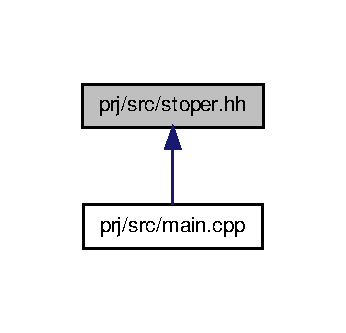
\includegraphics[width=166pt]{stoper_8hh__dep__incl}
\end{center}
\end{figure}
\subsection*{\-Komponenty}
\begin{DoxyCompactItemize}
\item 
class \hyperlink{classczas}{czas}
\end{DoxyCompactItemize}
\subsection*{\-Definicje}
\begin{DoxyCompactItemize}
\item 
\#define \hyperlink{stoper_8hh_a3d9fc3c745d0880902fe3ea3d5d5f71e}{\-C\-L\-O\-C\-K\-S\-\_\-\-P\-E\-R\-\_\-\-S\-E\-C}~1000000
\end{DoxyCompactItemize}


\subsection{\-Dokumentacja definicji}
\hypertarget{stoper_8hh_a3d9fc3c745d0880902fe3ea3d5d5f71e}{\index{stoper.\-hh@{stoper.\-hh}!\-C\-L\-O\-C\-K\-S\-\_\-\-P\-E\-R\-\_\-\-S\-E\-C@{\-C\-L\-O\-C\-K\-S\-\_\-\-P\-E\-R\-\_\-\-S\-E\-C}}
\index{\-C\-L\-O\-C\-K\-S\-\_\-\-P\-E\-R\-\_\-\-S\-E\-C@{\-C\-L\-O\-C\-K\-S\-\_\-\-P\-E\-R\-\_\-\-S\-E\-C}!stoper.hh@{stoper.\-hh}}
\subsubsection[{\-C\-L\-O\-C\-K\-S\-\_\-\-P\-E\-R\-\_\-\-S\-E\-C}]{\setlength{\rightskip}{0pt plus 5cm}\#define {\bf \-C\-L\-O\-C\-K\-S\-\_\-\-P\-E\-R\-\_\-\-S\-E\-C}~1000000}}\label{stoper_8hh_a3d9fc3c745d0880902fe3ea3d5d5f71e}


\-Definicja w linii 11 pliku stoper.\-hh.


\hypertarget{stos_8cpp}{\section{\-Dokumentacja pliku prj/src/stos.cpp}
\label{stos_8cpp}\index{prj/src/stos.\-cpp@{prj/src/stos.\-cpp}}
}
{\ttfamily \#include \char`\"{}stos.\-hh\char`\"{}}\*
\-Wykres zależności załączania dla stos.\-cpp\-:\nopagebreak
\begin{figure}[H]
\begin{center}
\leavevmode
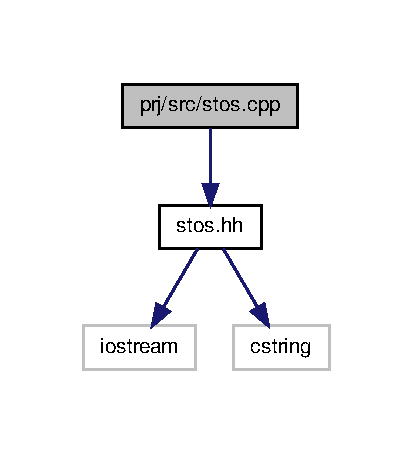
\includegraphics[width=198pt]{stos_8cpp__incl}
\end{center}
\end{figure}

\hypertarget{stos_8hh}{\section{\-Dokumentacja pliku prj/src/stos.hh}
\label{stos_8hh}\index{prj/src/stos.\-hh@{prj/src/stos.\-hh}}
}
{\ttfamily \#include $<$iostream$>$}\*
{\ttfamily \#include $<$cstring$>$}\*
\-Wykres zależności załączania dla stos.\-hh\-:\nopagebreak
\begin{figure}[H]
\begin{center}
\leavevmode
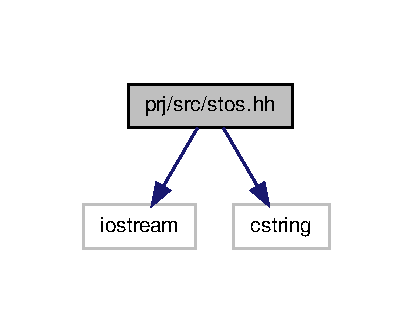
\includegraphics[width=198pt]{stos_8hh__incl}
\end{center}
\end{figure}
\-Ten wykres pokazuje, które pliki bezpośrednio lub pośrednio załączają ten plik\-:\nopagebreak
\begin{figure}[H]
\begin{center}
\leavevmode
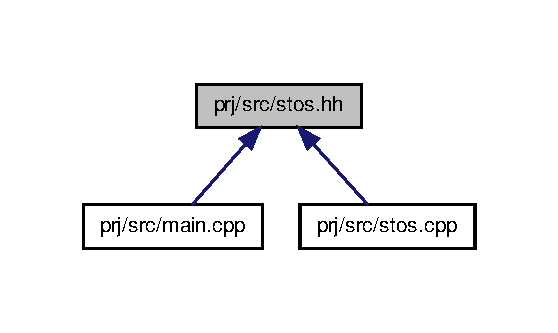
\includegraphics[width=268pt]{stos_8hh__dep__incl}
\end{center}
\end{figure}
\subsection*{\-Komponenty}
\begin{DoxyCompactItemize}
\item 
class \hyperlink{classstos}{stos}
\end{DoxyCompactItemize}
\subsection*{\-Definicje}
\begin{DoxyCompactItemize}
\item 
\#define \hyperlink{stos_8hh_acae4ff3359f7dda2fe2d2e82ec017d2c}{\-Z\-W\-I\-E\-K\-S\-Z}~zwieksz\-\_\-o\-\_\-1();
\begin{DoxyCompactList}\small\item\em wybor sposobu zwiekszania talicy ()-\/zwieksza dwukrotnie rozmiar tablicy ()-\/zwieksza o 1 rozmiar tablicy; \end{DoxyCompactList}\end{DoxyCompactItemize}


\subsection{\-Dokumentacja definicji}
\hypertarget{stos_8hh_acae4ff3359f7dda2fe2d2e82ec017d2c}{\index{stos.\-hh@{stos.\-hh}!\-Z\-W\-I\-E\-K\-S\-Z@{\-Z\-W\-I\-E\-K\-S\-Z}}
\index{\-Z\-W\-I\-E\-K\-S\-Z@{\-Z\-W\-I\-E\-K\-S\-Z}!stos.hh@{stos.\-hh}}
\subsubsection[{\-Z\-W\-I\-E\-K\-S\-Z}]{\setlength{\rightskip}{0pt plus 5cm}\#define {\bf \-Z\-W\-I\-E\-K\-S\-Z}~zwieksz\-\_\-o\-\_\-1();}}\label{stos_8hh_acae4ff3359f7dda2fe2d2e82ec017d2c}


\-Definicja w linii 16 pliku stos.\-hh.


\hypertarget{stos__lista_8cpp}{\section{\-Dokumentacja pliku prj/src/stos\-\_\-lista.cpp}
\label{stos__lista_8cpp}\index{prj/src/stos\-\_\-lista.\-cpp@{prj/src/stos\-\_\-lista.\-cpp}}
}
{\ttfamily \#include \char`\"{}stos\-\_\-lista.\-hh\char`\"{}}\*
\-Wykres zależności załączania dla stos\-\_\-lista.\-cpp\-:\nopagebreak
\begin{figure}[H]
\begin{center}
\leavevmode
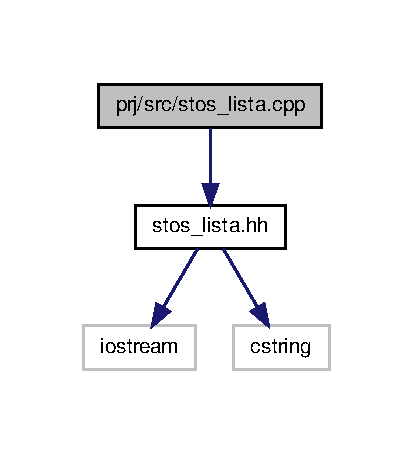
\includegraphics[width=198pt]{stos__lista_8cpp__incl}
\end{center}
\end{figure}

\hypertarget{stos__lista_8hh}{\section{\-Dokumentacja pliku prj/src/stos\-\_\-lista.hh}
\label{stos__lista_8hh}\index{prj/src/stos\-\_\-lista.\-hh@{prj/src/stos\-\_\-lista.\-hh}}
}
{\ttfamily \#include $<$iostream$>$}\*
{\ttfamily \#include $<$cstring$>$}\*
\-Wykres zależności załączania dla stos\-\_\-lista.\-hh\-:\nopagebreak
\begin{figure}[H]
\begin{center}
\leavevmode
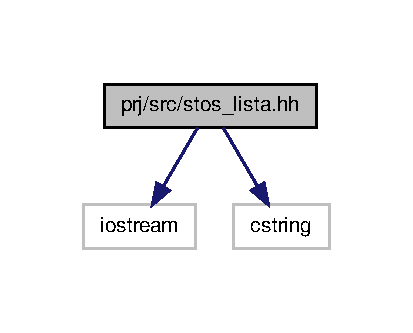
\includegraphics[width=198pt]{stos__lista_8hh__incl}
\end{center}
\end{figure}
\-Ten wykres pokazuje, które pliki bezpośrednio lub pośrednio załączają ten plik\-:\nopagebreak
\begin{figure}[H]
\begin{center}
\leavevmode
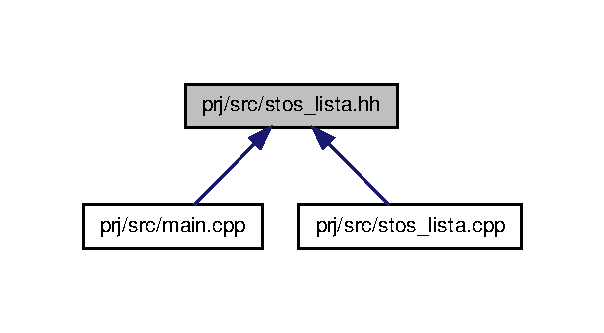
\includegraphics[width=290pt]{stos__lista_8hh__dep__incl}
\end{center}
\end{figure}
\subsection*{\-Komponenty}
\begin{DoxyCompactItemize}
\item 
struct \hyperlink{structelement}{element}
\item 
class \hyperlink{classstos__l}{stos\-\_\-l}
\end{DoxyCompactItemize}

\printindex
\end{document}
